\documentclass[a4paper,11pt]{article}
\pdfoutput=1 % if your are submitting a pdflatex (i.e. if you have
             % images in pdf, png or jpg format)

\usepackage{jheppub} % for details on the use of the package, please
                     % see the JHEP-author-manual

\usepackage[T1]{fontenc} % if needed
\usepackage{kotex}
\usepackage{hhline}

\title{\boldmath HW2 - Sanity Check and Determine dispersion relation with Oh et al.}


%% %simple case: 2 authors, same institution
%% \author{A. Uthor}
%% \author{and A. Nother Author}
%% \affiliation{Institution,\\Address, Country}

% more complex case: 4 authors, 3 institutions, 2 footnotes
\author{김태근, 윤한결, 강호철, 송진화}

% The "\note" macro will give a warning: "Ignoring empty anchor..."
% you can safely ignore it.

\affiliation{연세대학교 천문우주학과 F조}



\begin{document} 
\maketitle
\flushbottom

\section{Results}
\label{sec:result}

\subsection{Sanity Check}
\label{subsec:sanity}

\begin{table}[h]
\centering
\begin{tabular}{|c||c|c|c|c|c|c|c|c|c|c|c||c|}
\hline
Type & E & S0 & Sa & Sb & Sc & Sd & SBa & SBb & SBc & SBd & Sd & Total\\
\hhline{|=||=|=|=|=|=|=|=|=|=|=|=||=|}
Our data & 45 & 22 & 22 & 26 & 20 & 8 & 17 & 19 & 11 & 5 & 5 & 200\\
\hline
Matched data & 44 & 14 & 6 & 12 & 15 & 2 & 3 & 6 & 4 & 1 & 1 & 108\\
\hline
\end{tabular}
\caption{\label{tab:i} The number of our data \& matched data }
\end{table}


\begin{figure}[h]
\centering
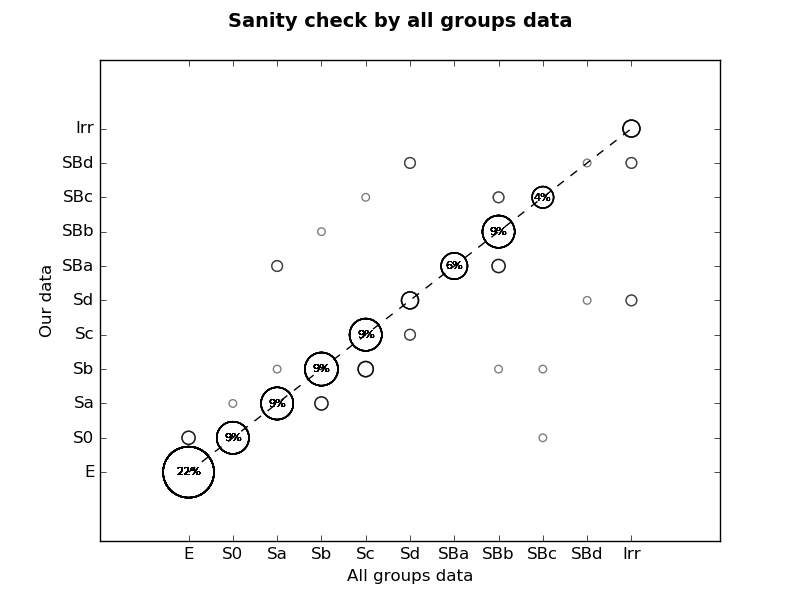
\includegraphics[height=60mm, width=100mm]{Sanity.png}
\hfill
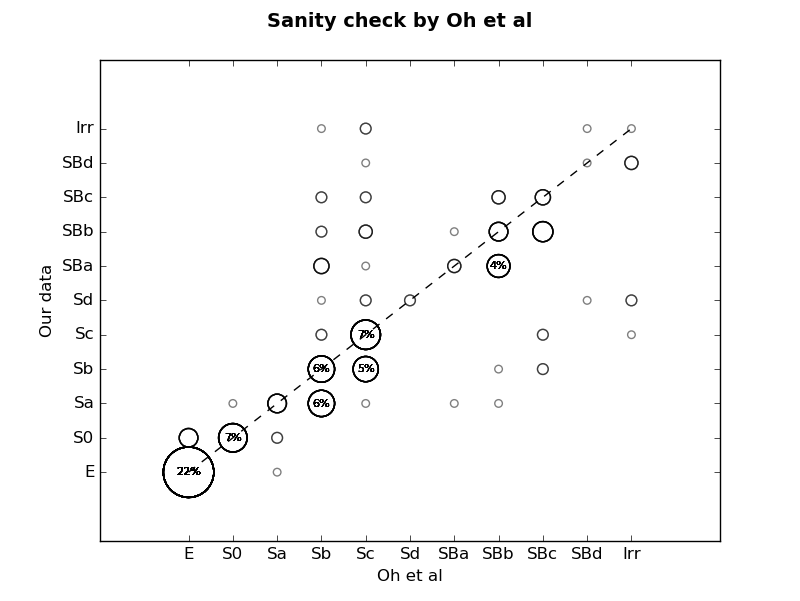
\includegraphics[height=60mm, width=100mm]{Sanity_oh.png}
\caption{\label{fig:i} Sanity check by all groups' data and Oh et al.}
\end{figure}

\subsection{Dispersion Relation}
\label{subsec:disp}

\begin{table}[h]
\centering
\begin{tabular}{|c||c|c|c|c|c|c|c|c|c|c|c||c|}
\hline
Type & E & S0 & Sa & Sb & Sc & Sd & SBa & SBb & SBc & SBd & Irr & Total\\
\hhline{|=||=|=|=|=|=|=|=|=|=|=|=||=|}
Dist & 0.009 &0.037&0.054&0.048&0.017&0.023&0.049&0.042&0.020&0.014&0.029&0.344\\
\hline
\end{tabular}
\caption{\label{tab:ii} Distance of our data for each type}
\end{table}

\begin{table}[h!]
\centering
\begin{tabular}{|c||c|c|c|c|c|c|c|c|c|c|c|c|}
\hline
Group & Oh & A & B & C & D & E & F & G & H & I & J \\
\hhline{|=||=|=|=|=|=|=|=|=|=|=|=|}
Dist & 0 &
0.512&0.345&0.362&0.348&0.568&0.344&0.389&0.422&0.361&0.270\\
\hline
Rank &1&10&4&7&5&11&3&8&9&6&2\\
\hline
\end{tabular}
\caption{\label{tab:iii} Distance of all groups}
\end{table}

\begin{figure}[h!]
\centering
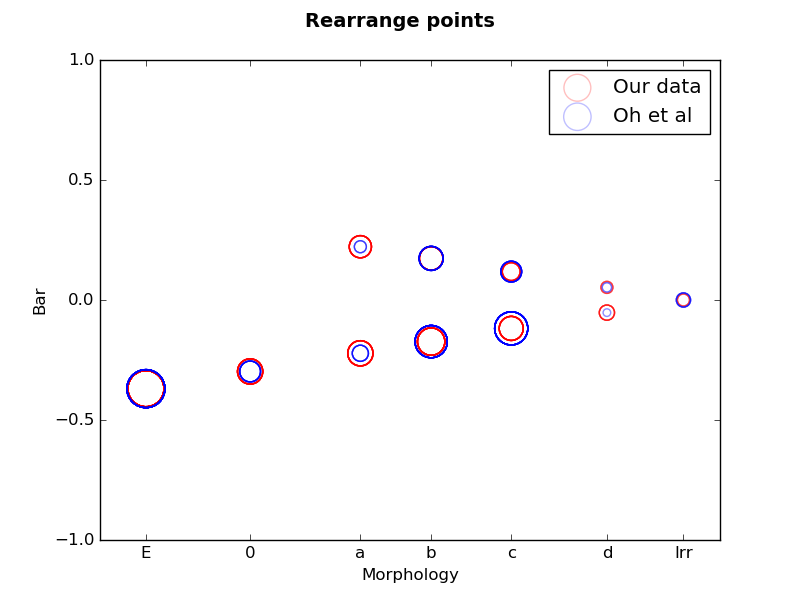
\includegraphics[height=65mm, width=100 mm]{Rearrange_final.png}
\caption{\label{fig:ii} Rearrange points by our criteria}
\end{figure}

\newpage


\section{Discussion}
\subsection{Sanity Check}


Sanity check는 두 번 진행하였는데, 먼저 다른 조 학생들의 분류 data만 가지고 F조의 분류 결과와 비교하였고, 두 번째로 학생들 전체+Oh et al. 2013 과의 비교를 진행하였다(Fig:\ref{fig:i}). 두 번째 분류를 진행한 이유는 우리의 분류가 'trained eye'의 분류와 얼마나 많이 다른가를 보기 위함이다. 다른 조의 분류와 비교했을 때, 놀랍게도 거의 모든 은하의 분류가 비슷한 것을 확인 할 수 있었다. 5% 이상의 차이를 보이는 분류는 나오지 않았으며, 대부분의 차이가 Sa와 SBa처럼 bar의 유무, 또는 b와 c 사이의 구별과 같은 약간의 차이만이 있었다. 
하지만 Oh et al.과의 sanity 체크는 조금 더 큰 편차를 보였다. 나선은하의 분류(특히 Sb와 Sc)에서 큰 차이가 있었으며, 단순히 bar의 유무만 차이를 보인 것이 아니라 S0에서부터 SBd까지 넓은 범위에서 다른 분류를 한 것을 확인할 수 있었다.

\subsection{Determine distance of x-axis}



F조의 분류 결과를 다른 조의 분류 결과나 Oh et al.에서의 분류와 비교하기 위해서 x축을 morphological type (E, S0, S(B)a,S(B)b,S(B)c,S(B)d Irr)로 나누고 y축을 Bar의 유무(Bar, Irr, No Bar)로 나누었다. 그 다음, 각 조의 분류를 좌표에 대입한 뒤, 각 좌표간의 거리를 평균내어 분류 결과의 차이를 나타내고자 했다.
 이러한 방식에서 가장 중요한 것은 각 기준마다의 x축, y축 간의 거리를 설정하는 것이었다. 우선 x축 사이의 거리(e.g. E와 S0와의 거리, S0와 S(B)a와의 거리, etc.)를 결정하는 방식은 모든 조의 결과를 분석하여 서로 어떤 Type 간에 헷갈림이 심했는 지를 분석하여 헷갈리는 정도가 심했을 경우 그 거리를 적게 하기로 조정했다. 이 과정을 정확히 서술하자면, 10개 조의 분류(Untrained Eye의 분류)와 Oh et al.(Trained Eye의 분류)를 비교하여 각 분류의 차이를 분석하여 서로 다르게 표현한 수 (Fig:\ref{fig:iii}) 를 전체 분류의 수로 나누어 일종의 '헷갈림 확률'을 구하였다. 이 확률값에 1을 빼서 이 값을 x축 사이의 거리로 설정하였다. 이를 사용하여 헷갈릴 확률이 높은 Type의 경우 x축 사이의 거리가 적기 때문에 다른 Type간의 헷갈림 보다 그 차이가 적어지도록 했다. (Table:\ref{tab:iv})
 
 이렇게 구한 최종 Index를 확인해본 결과 a-b의 경우 그 헷갈림 정도가 제일 심했던 것을 확인할 수 있었다. arm tightness, bulge의 크기 등을 종합적으로 고려해야 하는 나선 은하의 분류의 경우 Untrained Eye인 학생들에겐 차이가 일어난 것을 확인할 수 있었고 S0-S(B)a의 경우 Disk와 Arm의 존재를 확인할 경우 구분이 가능했기 때문에 Untrained Eye에게도 구분을 쉽게 할 수 있었던 것으로 보인다.


\subsection{Determine distance of y-axis}

헷갈림 정도 수치 설정에 있어, 먼저 그 크기는 앞서 설명한 것 처럼 통계적 접근으로 그 수치를 결정하였다. 그러나 토의 결과 Sa, Sb, Sc, Sd 사이의 차이나 Bar가 존재하는 SBa, SBb, SBc, SBd 사이의 구분과 Bar의 존재 구분은 그 관계에 있어서 다른 성질의 것이었기에 축을 나누어 두 가지로 생각해 볼 필요가 있게 되었다. 쉽게 말해서 Sa가 Sb와 착각되는 것과는 별개로 SBa와 잘못 판단되는 결과를 이번 분포를 통해 확인하였기에 여기에도 수치의 조정이 필요함을 확인했다는 것이다. 그래서 이번 논의에서는 Bar-Index라는 개념을 도입하여 Bar와 Non-bar galaxy 사이의 confusion rate를 고려해 주었다. 

이 헷갈림 확률을 고려하여 bar 사이의 거리를 interpolation 한 결과는 다음 분포를 보인다(Fig:\ref{fig:iv}). a의 경우는 원 데이터를 여러모로 분석해 본 결과 통계적 오류로 판단되어 이를 제외하였다. 그렇게 하면 결국 이런 linear한 분포를 볼 수 있는데, 여기에 앞서 설명한 x축 방향으로의 헷갈림 확률을 고려한 차이를 넣어주면 exponential한 분포의 모습이 됨을 확인할 수 있다. 그런데 여기에서도 논의가 더 이루어졌는데, Bar-Index에서의 거리는 어떻게 구하느냐에 그 논의의 초점이 만들어졌다. exponential한 분포를 보이는 것에는 모두가 동의했으나 그 정도는 어떻게 정하느냐는 문제에 빠졌는데, 이는 가장 많은 데이터를 가지고 있는 Sb에서 이들이 Sa, Sc, Sd와 헷갈리는 정도와 SBb와 헷갈리는 정도의 비를 통해 그 비로 Sb에서의 Bar-Index의 크기를 결정하고 이 점을 기준으로 조금 전에 설정한 expoenetial 분포를 적용하는 것으로 하였다. 원래라면 각각의 데이터에 대해 같은 방법을 사용해야 했지만, Sd, SBd의 경우 그 data가 적어 특히 Sd와 SBd에서의 confusion rate는 의미가 없다고 판단하여 이를 확대 적용하였다.

\appendix
\section{Confusion index}
\label{sec:confuse}

\begin{figure}[h!]
\centering
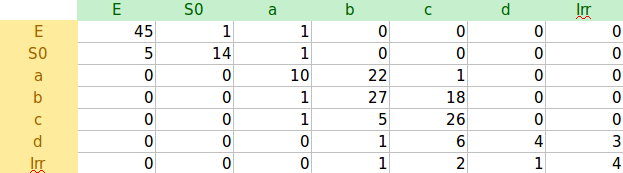
\includegraphics[height=20mm, width=100 mm]{Dobby.png}
\caption{\label{fig:iii} The number of confusion}
\end{figure}



\begin{table}[h]
\centering
\begin{tabular}{|c|c|c|c|c|c|}
\hline
E-S0 &	S0-a & a-b & b-c & c-d	& d-Irr\\
\hline
0.91 & 0.96 & 0.6166666667  & 0.6973684211	& 0.8333333333	& 0.6666666667\\
\hline
\end{tabular}
\caption{\label{tab:iv} Confusion Index }
\end{table}

\section{Interpolation of distance of bar}
\label{sec:interp}

\begin{figure}[h!]
\centering
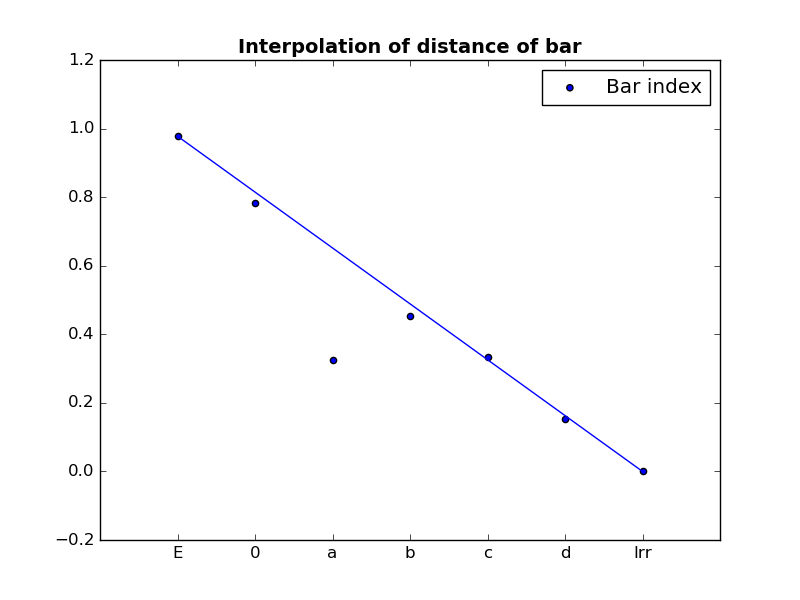
\includegraphics[height=50mm, width=90 mm]{interpolation.png}
\caption{\label{fig:iv} Interpolation of bar-distance}
\end{figure}


\end{document}
